\documentclass[conference]{IEEEtran}
\IEEEoverridecommandlockouts
\usepackage{cite}
\usepackage{amsmath,amssymb,amsfonts}
\usepackage{algorithmic}
\usepackage{algorithm}
\usepackage{graphicx}
\graphicspath{{figures/}}
\usepackage{textcomp}
\usepackage{xcolor}
\usepackage{booktabs}
\usepackage{multirow}
\usepackage{url}
\usepackage{microtype}

\def\BibTeX{{\rm B\kern-.05em{\sc i\kern-.025em b}\kern-.08em
    T\kern-.1667em\lower.7ex\hbox{E}\kern-.125emX}}

\begin{document}

\title{EvoSynth: Dynamic Multi-Armed Bandit Meta-Optimizer for Automated Hyperparameter Tuning and Model Selection\\
\thanks{Project Group: G002. Capstone Engineering Research Project.}
}

\author{
\IEEEauthorblockN{Group G002}
\IEEEauthorblockA{\textit{Department of Computer Science and Engineering} \\
\textit{College of Engineering and Technology}\\
Email: project.g002@college.edu}
}

\maketitle

\begin{abstract}
No single hyperparameter optimizer performs best on every problem, yet most tuners commit their whole budget to one search algorithm chosen in advance. This paper presents \textbf{EvoSynth}, an AutoML meta-optimizer that runs a portfolio of four population-based optimizers---Genetic Algorithm (GA), Particle Swarm Optimization (PSO), Differential Evolution (DE) and CMA-ES---in a two-tier island model and reallocates the budget among them online with a UCB1 multi-armed bandit. Model family, feature-engineering strategy and hyperparameters are encoded together in one continuous latent space $[0,1]^d$, so every optimizer searches the combined model-selection and tuning problem. A five-term composite score (fitness, speed, efficiency, diversity, trend) drives promotion of the two strongest optimizers, live swaps with rollback, elite sharing between families and diversity injection on stagnation. After the search, the five best distinct configurations are re-scored with 5-fold cross-validation, and the selected one is refitted once and scored once on held-out test rows. We evaluate EvoSynth against untuned models, Random Search, Optuna TPE and FLAML on UCI Covertype and Adult under an identical protocol. With 500 evaluations EvoSynth reached 93.89\% test accuracy on Covertype and 92.96 ROC AUC on Adult, level with Random Search and Optuna (within 0.03 points), 1.4 points above FLAML on Covertype and 0.17 below it on Adult, while selecting a different model family for each dataset. In an ablation it matched the best of the four optimizers run alone without knowing in advance which one that would be. Parallel evaluation gave a measured $6.1\times$ speed-up on 12 threads. The same engine also searches CNN architectures (81.8\% validation accuracy on Fashion-MNIST in 160 evaluations).
\end{abstract}

\begin{IEEEkeywords}
Hyperparameter Optimization, Automated Machine Learning, Algorithm Selection, Multi-Armed Bandit, UCB1, Genetic Algorithm, Particle Swarm Optimization, Differential Evolution, CMA-ES, Island Model.
\end{IEEEkeywords}

\section{Introduction}
Model performance depends heavily on hyperparameters such as learning rate, tree depth, number of estimators and regularization strength, which are not learned during training \cite{feurer2019hyperparameter}. Choosing the model family and the feature preprocessing is part of the same problem, known as combined algorithm selection and hyperparameter optimization (CASH).

Common approaches each have a drawback:
\begin{enumerate}
    \item \textbf{Grid and random search} ignore feedback from earlier evaluations; random search is nevertheless a strong baseline in low effective dimensions \cite{bergstra2012random}.
    \item \textbf{Single-strategy optimizers} (Bayesian optimization with TPE \cite{bergstra2011algorithms} or SMAC \cite{hutter2011sequential}, or one evolutionary algorithm) commit to one search behaviour. By the No Free Lunch theorem \cite{wolpert1997no}, no single strategy is best on every landscape, and the best one for a given dataset is not known in advance.
    \item \textbf{Post-hoc ensembles} (H2O AutoML \cite{ledell2020h2o}, AutoGluon) combine many trained models at prediction time, which multiplies inference latency and memory.
\end{enumerate}

\begin{figure*}[t]
\centering
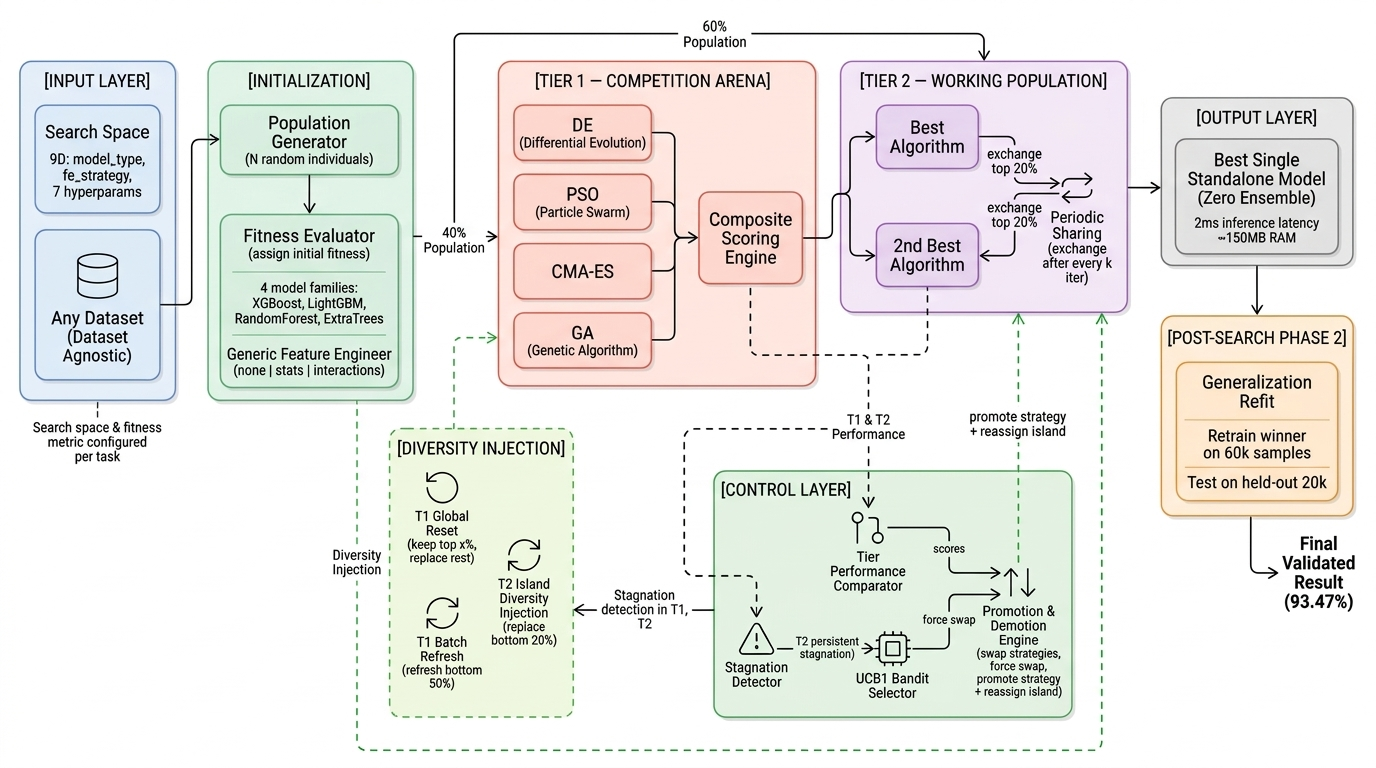
\includegraphics[width=\textwidth]{arch.png}
\caption{EvoSynth architecture for a population of $N$: (1) input layer and latent space; (2) parallel evaluation of the initial population and a stratified split into Tier 1 (40\%, four islands of $N/10$) and a reserve (60\%, two groups); (3) Tier 1 competition of GA, PSO, DE and CMA-ES; (4) composite scoring; (5) control layer with UCB1 bandit, promotion, SWAP and rollback; (6) Tier 2 working population with pairwise elite sharing; (7) diversity injection; (8) output: confirm before select, one refit, and a single model scored on held-out test rows.}
\label{fig:architecture}
\end{figure*}

\subsection{The EvoSynth Approach}
EvoSynth treats the choice of search algorithm as an online decision. It runs four complementary population-based optimizers:
\begin{itemize}
    \item \textbf{GA}: tournament selection, crossover and mutation for broad exploration.
    \item \textbf{PSO} \cite{kennedy1995particle}: particles pulled toward personal and global bests, fast on smooth regions.
    \item \textbf{DE} \cite{storn1997differential}: DE/rand/1/bin with one-to-one replacement, robust exploration through difference vectors.
    \item \textbf{CMA-ES} \cite{hansen2001completely}: adapts a covariance matrix for fine-tuning.
\end{itemize}
A UCB1 bandit \cite{auer2002finite} over these families, in the spirit of bandit-based adaptive operator selection \cite{fialho2010analyzing}, gives more of the budget to whichever family is making progress on the current problem, and good solutions are shared between families. The output is a single model, so serving it costs no more than serving that model alone.

The contributions of this work are: (i) a two-tier island portfolio of four evolutionary and swarm optimizers controlled by a UCB1 bandit over a five-term composite score; (ii) a single latent encoding of model family, feature engineering and hyperparameters; (iii) an evaluation protocol with fixed held-out test rows, confirm-before-select and an identical refit for every tuned method, published as EvoSynth-Bench v2.0.0; and (iv) a measured comparison with Random Search, Optuna and FLAML, an optimizer ablation, a speed-up benchmark and inference-cost measurements.

\section{System Workflow and Architecture}
Fig.~\ref{fig:architecture} shows the pipeline. Every random number generator is seeded from one run seed, so a run can be repeated exactly.

\subsection{Stage 1: Universal Latent Space}
The tabular search space has eight dimensions: model family (XGBoost \cite{chen2016xgboost}, RandomForest, LightGBM \cite{ke2017lightgbm}, ExtraTrees), feature-engineering strategy (none, row statistics, pairwise interactions), learning rate $[0.01, 0.3]$ (log scale), number of estimators $[50, 500]$, maximum depth $[3, 10]$, subsample $[0.5, 1]$, column-sample ratio $[0.3, 1]$ and L1 regularization $[0, 10]$. Each dimension $j$ is represented by $z_j \in [0, 1]$. Continuous parameters are decoded linearly or logarithmically,
\begin{equation}
x_j = L_j + z_j (U_j - L_j),
\end{equation}
and a choice with $K$ options takes the bin
\begin{equation}
k = \min(\lfloor z_j K \rfloor, K - 1).
\end{equation}
All four optimizers therefore work on the same continuous vectors. Hyperparameters that the decoded model does not use (for example the learning rate for ExtraTrees) are carried but inactive.

\subsection{Stage 2: Initial Population and Tier Split}
A random population of $N$ vectors (40 in our experiments) is evaluated in parallel. Each candidate is scored by stratified 2-fold cross-validation on the dataset's search rows, in the dataset's metric (accuracy or ROC AUC); gradient-boosted models stop early on a 15\% slice of the training fold. The population is then split by a stratified draw: the ranked population is cut into strata, and each Tier 1 island and reserve group receives members from every stratum. Tier 1 receives 40\% as four equal islands of $N/10$, one per optimizer; the remaining 60\% is held in reserve as two groups.

\subsection{Stage 3: Tier 1 Competition}
The four optimizers run for $T_1$ iterations through an ask/tell interface: \texttt{ask($n$)} proposes $n$ vectors and \texttt{tell($\cdot$)} returns their scores. A Tier 1 island whose best does not improve between iterations has 50\% of its members replaced by random vectors through the optimizer's \texttt{inject} method, which also updates its internal state (velocities, covariance, DE targets).

\subsection{Stage 4: Composite Scoring}
Each family $i$ is scored on five terms, each min--max normalised across the competing families:
\begin{equation}
C_i = 0.30 F_i + 0.25 S_i + 0.15 E_i + 0.15 D_i + 0.15 T_i,
\end{equation}
where $F_i$ is the family's best cross-validated score, $S_i$ (speed) the improvement of that best since the family's previous scoring call, $E_i$ (efficiency) that improvement per second of evaluation time, $D_i$ the mean pairwise distance between the island's latent vectors divided by $\sqrt{d}$, and $T_i$ (trend) the slope of the best score over the last three scoring calls. A family that is still improving can therefore outrank one with a slightly higher but stalled best.

\subsection{Stage 5: UCB1 Control Layer}
The bandit adds an exploration bonus to the composite score:
\begin{equation}
U_i = C_i + c\sqrt{\frac{\ln N_{\text{total}}}{n_i}}, \quad c = 0.1,
\end{equation}
where $N_{\text{total}}$ is the number of evaluations used and $n_i$ the number used by family $i$. After Tier 1, the two families with the highest $U_i$ are promoted to Tier 2, each taking one reserve group. Every $k$ Tier 2 iterations (a checkpoint; $k$ is chosen automatically so that Tier 2 has at least two checkpoints), the controller compares tiers: if the best Tier 1 family's $U$ exceeds the weaker Tier 2 family's by more than 0.10, the two are swapped. If the promoted family does not improve the global best within a 5-iteration grace period, the swap is rolled back from a saved snapshot, and cooldowns prevent immediate re-swapping. Every promotion, swap, rollback, injection and elite exchange is recorded.

\subsection{Stage 6: Tier 2 and Elite Sharing}
At each checkpoint the two Tier 2 islands trade elites pairwise: the worst 20\% of each island are replaced by the best 20\% of the other. This moves good configurations between algorithm families, for example a region found by CMA-ES into the GA population.

\subsection{Stage 7: Diversity Injection}
A Tier 2 island that stays stagnant for three consecutive checkpoints has its worst 20\% replaced by random vectors, again through \texttt{inject}.

\subsection{Stage 8: Confirm, Refit and Measure}
Two-fold scores are noisy, and the maximum of many noisy scores is biased upwards. EvoSynth therefore re-scores the five best distinct configurations with 5-fold CV on the search rows and selects the best confirmed one. That configuration is refitted on the dataset's train rows and scored once on the held-out test rows, which no search or selection step ever sees. Its single-row latency (one thread), batch throughput and serialized size are measured on the test rows.

\begin{algorithm}[t]
\caption{EvoSynth optimization lifecycle}
\label{alg:evosynth}
\begin{algorithmic}[1]
\REQUIRE Space $\mathcal{S}$, evaluator $\mathcal{E}$, budget $B$, population $N$, Tier 1 iterations $T_1$, checkpoint interval $k$
\STATE $\mathcal{P} \leftarrow$ $N$ random vectors; evaluate $\mathcal{P}$ in parallel
\STATE Stratified split: four Tier 1 islands (40\%) and two reserve groups (60\%)
\FOR{$t = 1$ \TO $T_1$}
    \STATE Each optimizer: ask, evaluate in parallel, tell; inject 50\% if stagnant
\ENDFOR
\STATE Score families ($C_i$, $U_i$); promote the top two, each with one reserve group
\WHILE{evaluations used $< B$}
    \STATE Step every Tier 2 and Tier 1 optimizer
    \IF{checkpoint (every $k$ iterations)}
        \STATE Rescore; SWAP if $U_{\text{T1}} > U_{\text{T2,weak}} + 0.10$
        \STATE Pairwise elite sharing between the Tier 2 islands
        \STATE Inject 20\% into Tier 2 islands stagnant for 3 checkpoints
    \ENDIF
    \STATE Roll back a swap whose grace period ends without a new global best
\ENDWHILE
\STATE Confirm the top 5 distinct configurations with 5-fold CV; select the best
\RETURN Refitted model, test score and inference cost
\end{algorithmic}
\end{algorithm}

\section{Experimental Evaluation}

\subsection{Setup}
\textbf{Datasets.} UCI Forest Covertype \cite{blackard1999comparative} (581,012 rows, 54 features, 7 imbalanced classes; accuracy) and Adult \cite{kohavi1996scaling} (48,842 rows, 14 features, binary; ROC AUC). Each dataset is split once: test rows are set aside first (Covertype 20,000; Adult 12,000), then search rows and train rows (Covertype 60,000; Adult 36,000) are drawn from the rest. Searches used a fixed 10,000-row subset of the search rows. The exact row indices are published in EvoSynth-Bench v2.0.0 (doi:10.5281/zenodo.23645119).

\textbf{Methods.} EvoSynth (population 40, 500 evaluations, 8 parallel workers); Random Search and Optuna TPE \cite{akiba2019optuna} (500 trials each, same space and evaluator, sequential); FLAML \cite{wang2021flaml} with the wall time EvoSynth used, searching on the train rows with its own holdout and fitting its own final model; and each model family with library defaults. EvoSynth, Random Search and Optuna use the same confirm-before-select step and the same refit, so their test scores are directly comparable.

\textbf{Hardware and seeds.} One 12-thread laptop CPU. All results are from seed 42; differences of a few tenths of a point between tuned methods should be read as ties until repeated over seeds.

\subsection{Main Comparison}
Table~\ref{tab:main} gives the held-out test scores. On both datasets EvoSynth, Random Search and Optuna finish within 0.03 points of each other and choose the same model family: ExtraTrees with interaction features on Covertype and XGBoost on Adult. Tuning with model selection is worth 4.1 points over the best untuned model on Covertype but only 0.06 on Adult, where default LightGBM is already near the top. FLAML is 1.4 points lower on Covertype and best on Adult (+0.17). EvoSynth's search took 12 minutes on Covertype against 42--50 minutes for the sequential baselines; on Adult, where an evaluation takes about a second, Optuna was about as fast (3.3 against 3.0 minutes).

\begin{table}[htbp]
\caption{Held-out test score (seed 42; 500 evaluations for tuned searches)}
\label{tab:main}
\centering
\setlength{\tabcolsep}{4pt}
\begin{tabular}{lcccc}
\toprule
 & \multicolumn{2}{c}{\textbf{Covertype (acc.\,\%)}} & \multicolumn{2}{c}{\textbf{Adult (AUC\,\%)}} \\
\textbf{Method} & \textbf{Test} & \textbf{Time} & \textbf{Test} & \textbf{Time} \\
\midrule
Untuned XGBoost & 85.58 & -- & 92.70 & -- \\
Untuned LightGBM & 84.69 & -- & 92.92 & -- \\
Untuned RandomForest & 89.09 & -- & 90.74 & -- \\
Untuned ExtraTrees & 89.77 & -- & 89.15 & -- \\
FLAML & 92.53 & 13.0\,m & \textbf{93.13} & 3.0\,m \\
Random Search & \textbf{93.89} & 42.4\,m & 92.98 & 19.1\,m \\
Optuna TPE & 93.87 & 49.8\,m & 92.95 & 3.3\,m \\
\textbf{EvoSynth} & \textbf{93.89} & 12.2\,m & 92.96 & 3.0\,m \\
\bottomrule
\end{tabular}
\end{table}

Test scores exceed search scores on Covertype (82.35\% with 2-fold CV on 10,000 rows, 84.84\% after 5-fold confirmation) because the refit trains on 60,000 rows; the test rows are never seen before the final score.

\textbf{A plateau in the search space.} The five best Covertype configurations scored exactly 82.35\% in search and 84.84\% in confirmation. During the search, forests are capped at 150 trees, depth is mapped to three times the gene value, and the column-sample ratio is rounded to a whole number of features, so these different vectors build the same model. Every competent method reaches this plateau, which explains the ties on Covertype; datasets where continuous boosting hyperparameters matter are better suited to separating optimizers.

\subsection{Optimizer Ablation}
Each optimizer was run alone with the full 500-evaluation budget and population 40, and EvoSynth was run once with the same budget; all five were scored by the same composite engine at fixed marks (Table~\ref{tab:ablation}). EvoSynth matched the best single optimizer at the full budget (82.35\%, tied with PSO and CMA-ES) and trailed PSO by 0.27 points at the 25\% mark. The best single optimizer differs between runs (CMA-ES and DE in our earlier ablations, PSO here), so the portfolio's value is that it reaches the best score without that choice being made in advance. GA alone collapsed (diversity 0.085) and was the weakest; inside EvoSynth, GA produced the winning configuration after receiving CMA-ES's elites.

\begin{table}[htbp]
\caption{Ablation on Covertype: best search CV accuracy (\%)}
\label{tab:ablation}
\centering
\begin{tabular}{lcccc}
\toprule
\textbf{Method} & \textbf{@125} & \textbf{@500} & \textbf{Diversity} & \textbf{Time} \\
\midrule
GA alone & 81.53 & 82.21 & 0.085 & 14.9\,m \\
PSO alone & 82.35 & 82.35 & 0.093 & 10.7\,m \\
DE alone & 82.13 & 82.34 & 0.363 & 9.8\,m \\
CMA-ES alone & 81.89 & 82.35 & 0.227 & 10.5\,m \\
\textbf{EvoSynth} & 82.08 & \textbf{82.35} & 0.206 & 14.9\,m \\
\bottomrule
\end{tabular}
\end{table}

\subsection{Meta-Decisions in Practice}
In the Covertype search, DE and CMA-ES were promoted after Tier 1. DE had a lower best score than CMA-ES but the highest composite score, because it was still improving and had the most diverse island. At the first checkpoint GA, which was improving quickly from a low score, displaced DE by a SWAP (UCB 0.592 against 0.369). GA reached the 82.35\% plateau through CMA-ES's shared elites but did not improve the global best in its grace period, so the swap was rolled back and DE restored. CMA-ES found the winning configuration. In the Adult search GA and PSO were promoted, two swaps followed, and PSO found the winner. The family that produced the winner differed in every run (CMA-ES, PSO, and GA in the ablation).

\subsection{Speed-Up}
The same 40 random Covertype configurations were evaluated under four conditions (Table~\ref{tab:speedup}). Parallel evaluation on 12 threads gave $5.85\times$; early stopping added little ($1.17\times$ alone, $6.10\times$ combined) and lowered the mean CV score by 0.37 points. Parallel evaluation is available to other tuners as well, so this is an engineering gain rather than a property of the search method.

\begin{table}[htbp]
\caption{Time to evaluate 40 Covertype configurations}
\label{tab:speedup}
\centering
\begin{tabular}{lcc}
\toprule
\textbf{Condition} & \textbf{Time (s)} & \textbf{Speed-up} \\
\midrule
Sequential & 255.6 & 1.00$\times$ \\
Sequential + early stopping & 219.0 & 1.17$\times$ \\
Parallel, 12 threads & 43.7 & 5.85$\times$ \\
\textbf{Parallel + early stopping} & \textbf{41.9} & \textbf{6.10$\times$} \\
\bottomrule
\end{tabular}
\end{table}

\subsection{Inference Cost}
The cost of the delivered model depends on the family selected. The Covertype winner, a 232-tree ExtraTrees with interaction features, takes 12.5\,ms per row on one thread and occupies 470\,MB; the Adult winner, an XGBoost, takes 0.26\,ms and 0.4\,MB. A single model avoids the multiplication of cost that a stacked ensemble incurs, but EvoSynth does not currently trade accuracy for size or latency.

\subsection{Neural Architecture Search}
As in neural architecture search \cite{zoph2016neural, real2019regularized}, the same engine searched a CNN space (channel counts, fully connected units, dropout, activation, optimizer and learning rate) on Fashion-MNIST \cite{xiao2017fashion}, training each candidate for two epochs on 10,000 images. With 160 evaluations it reached 81.8\% validation accuracy (conv 16--128, fc 256, ReLU, Adam), found by PSO in Tier 2, with no code changes to the engine.

\section{Real-Time Glass-Box Telemetry Dashboard}
The controller emits structured events over Server-Sent Events from a FastAPI server: evaluation metrics, composite and UCB scores, tier assignments, and every meta-decision (promotion, swap, rollback, injection, elite sharing). A React dashboard displays live score curves, tier membership, composite breakdowns and the decision log, so a user can see why the budget moved between optimizers.

\section{Conclusion}
EvoSynth coordinates four evolutionary and swarm optimizers through a two-tier island model and a UCB1 bandit over a composite score, searching model family, feature engineering and hyperparameters in one latent space and delivering a single model. Under an identical protocol with held-out test rows, it matched Random Search and Optuna on Covertype and Adult, selected the right model family for each, and matched the best single optimizer in an ablation without knowing which one that would be; parallel evaluation made it the fastest tuned search on Covertype. The results also show its limits: on these datasets it does not beat strong baselines, FLAML was best on Adult, and the Covertype search space contains a plateau that every competent method reaches. Future work will repeat the experiments over multiple seeds and harder datasets (HIGGS, Poker Hand), compare against portfolio baselines such as Nevergrad's NGOpt on surrogate benchmarks with many tasks, use rank-normalised rewards, and add size- and latency-aware objectives.

\begin{thebibliography}{00}
\bibitem{feurer2019hyperparameter} M. Feurer and F. Hutter, ``Hyperparameter optimization,'' in \textit{Automated Machine Learning}, Springer, Cham, 2019, pp. 3--33.
\bibitem{bergstra2012random} J. Bergstra and Y. Bengio, ``Random search for hyper-parameter optimization,'' \textit{Journal of Machine Learning Research}, vol. 13, no. 2, pp. 281--305, 2012.
\bibitem{auer2002finite} P. Auer, N. Cesa-Bianchi, and P. Fischer, ``Finite-time analysis of the multiarmed bandit problem,'' \textit{Machine Learning}, vol. 47, no. 2, pp. 235--256, 2002.
\bibitem{kennedy1995particle} J. Kennedy and R. Eberhart, ``Particle swarm optimization,'' in \textit{Proceedings of ICNN'95 - International Conference on Neural Networks}, vol. 4, 1995, pp. 1942--1948.
\bibitem{storn1997differential} R. Storn and K. Price, ``Differential evolution--a simple and efficient heuristic for global optimization over continuous spaces,'' \textit{Journal of Global Optimization}, vol. 11, no. 4, pp. 341--359, 1997.
\bibitem{hansen2001completely} N. Hansen and A. Ostermeier, ``Completely derandomized self-adaptation in evolution strategies,'' \textit{Evolutionary Computation}, vol. 9, no. 2, pp. 159--195, 2001.
\bibitem{chen2016xgboost} T. Chen and C. Guestrin, ``XGBoost: A scalable tree boosting system,'' in \textit{Proceedings of the 22nd ACM SIGKDD International Conference on Knowledge Discovery and Data Mining}, 2016, pp. 785--794.
\bibitem{ke2017lightgbm} G. Ke et al., ``LightGBM: A highly efficient gradient boosting decision tree,'' in \textit{Advances in Neural Information Processing Systems}, vol. 30, 2017.
\bibitem{fialho2010analyzing} A. Fialho, L. Da Costa, M. Schoenauer, and M. Sebag, ``Analyzing bandit-based adaptive operator selection mechanisms,'' \textit{Annals of Mathematics and Artificial Intelligence}, vol. 60, no. 1, pp. 25--64, 2010.
\bibitem{bergstra2011algorithms} J. Bergstra, R. Bardenet, Y. Bengio, and B. K{\'e}gl, ``Algorithms for hyper-parameter optimization,'' in \textit{Advances in Neural Information Processing Systems}, vol. 24, 2011.
\bibitem{wang2021flaml} C. Wang, Q. Wu, M. Weimer, and E. Zhu, ``FLAML: A fast and lightweight AutoML library,'' \textit{Proceedings of Machine Learning and Systems}, vol. 3, pp. 434--447, 2021.
\bibitem{ledell2020h2o} E. LeDell and S. Poirier, ``H2O AutoML: Scalable automatic machine learning,'' in \textit{ICML Workshop on Automated Machine Learning}, 2020.
\bibitem{zoph2016neural} B. Zoph and Q. V. Le, ``Neural architecture search with reinforcement learning,'' in \textit{International Conference on Learning Representations (ICLR)}, 2017.
\bibitem{real2019regularized} E. Real, A. Aggarwal, Y. Huang, and Q. V. Le, ``Regularized evolution for image classifier architecture search,'' in \textit{AAAI Conference on Artificial Intelligence}, vol. 33, 2019, pp. 4780--4789.
\bibitem{hutter2011sequential} F. Hutter, H. H. Hoos, and K. Leyton-Brown, ``Sequential model-based optimization for general algorithm configuration,'' in \textit{International Conference on Learning and Intelligent Optimization}, Springer, 2011, pp. 507--523.
\bibitem{wolpert1997no} D. H. Wolpert and W. G. Macready, ``No free lunch theorems for optimization,'' \textit{IEEE Transactions on Evolutionary Computation}, vol. 1, no. 1, pp. 67--82, 1997.
\bibitem{akiba2019optuna} T. Akiba, S. Sano, T. Yanase, T. Ohta, and M. Koyama, ``Optuna: A next-generation hyperparameter optimization framework,'' in \textit{Proceedings of the 25th ACM SIGKDD International Conference on Knowledge Discovery and Data Mining}, 2019, pp. 2623--2631.
\bibitem{blackard1999comparative} J. A. Blackard and D. J. Dean, ``Comparative accuracies of artificial neural networks and discriminant analysis in predicting forest cover types from cartographic variables,'' \textit{Computers and Electronics in Agriculture}, vol. 24, no. 3, pp. 131--151, 1999.
\bibitem{kohavi1996scaling} R. Kohavi, ``Scaling up the accuracy of naive-Bayes classifiers: A decision-tree hybrid,'' in \textit{Proceedings of the Second International Conference on Knowledge Discovery and Data Mining (KDD)}, 1996, pp. 202--207.
\bibitem{xiao2017fashion} H. Xiao, K. Rasul, and R. Vollgraf, ``Fashion-MNIST: A novel image dataset for benchmarking machine learning algorithms,'' \textit{arXiv preprint arXiv:1708.07747}, 2017.
\end{thebibliography}

\end{document}
